% XAI drowsiness review. Compile on Overleaf: pdfLaTeX, then BibTeX, then pdfLaTeX twice.
% Upload this whole folder (main.tex, references.bib, sections/, figures/). IEEEtran is built into Overleaf.
\documentclass[journal]{IEEEtran}

\usepackage[utf8]{inputenc}
\usepackage[T1]{fontenc}
\usepackage{cite}
\usepackage{graphicx}
\usepackage{booktabs}
\usepackage{tabularx}
\usepackage{array}
\usepackage{url}
\usepackage{xcolor}
\usepackage[hidelinks]{hyperref}

\graphicspath{{figures/}}
\newcolumntype{Y}{>{\raggedright\arraybackslash}X}
\newcolumntype{L}[1]{>{\raggedright\arraybackslash}p{#1}}
% Visible reminders for the team. Search for \todo before submitting.
\newcommand{\todo}[1]{\textcolor{red}{[#1]}}

\begin{document}

\title{Explainable and Interpretable AI for Drowsiness Detection: A Cross-Modal Review and Critical Appraisal}

\author{Sunny Yadav, Akshay \todo{surname}, and Aryan \todo{surname}%
\thanks{The authors are with the Indian Institute of Technology Roorkee, India. \todo{department, supervisor, e-mail}}}

\maketitle

\begin{abstract}
Deep-learning drowsiness detectors are hard to trust in a vehicle because their decisions are opaque, and interpretable and explainable methods are offered as the remedy. We review 45 papers across electroencephalography (EEG), cardiac signals, camera-based vision, vehicle signals and multimodal fusion, classify them by how the explanation is produced and what it refers to, and appraise 41 detection studies on four checks: agreement with known physiology, a faithfulness test, testing on unseen drivers, and public code. Thirty-two studies report explanations at least partly consistent with known physiology, but only two tested faithfulness quantitatively, 28 did not evaluate the explanation, 15 clearly tested on unseen drivers, and five share code. Where explanations were tested they could disagree: attention and band ablation conflict in one EEG model, and four explainers rank differently on one alertness model. Several labels derive from model inputs or recording sessions, and median reported accuracy is 97.1\% under random or within-subject splits against 77.2\% on unseen drivers. A case study on a published interpretable EEG model shows that it outputs a constant class when normalisation cannot see the whole test subject, that changing only those statistics alters up to 24.6\% of decisions, that attribution methods strongest on deletion are weakest on a randomisation sanity check, and that the reading of alert decisions as artefacts holds weakly on the 11-subject subset but more clearly on all 27 subjects. We close with a reporting checklist. The papers came from targeted searches, so counts describe the examined set, not the field.
\end{abstract}

\begin{IEEEkeywords}
Drowsiness detection, driver monitoring, explainable artificial intelligence, interpretability, electroencephalography, heart rate variability, faithfulness, cross-subject validation.
\end{IEEEkeywords}

\section{Introduction}
\IEEEPARstart{D}{rowsy} driving remains a major road-safety problem. One recent survey cites a United States estimate attributing up to 20\% of annual traffic deaths in 2016 to driver drowsiness \cite{fu2024survey}. Automated detectors now use brain signals, heart signals, cameras and vehicle data, and reported accuracies often exceed 95\% under controlled conditions \cite{ajayi2025multimodal}.

High accuracy is not enough for a safety system. A driver, a manufacturer or a regulator needs to know why an alarm fired and whether the model relies on drowsiness itself or on an accident of the training data. Interpretable models and explainable artificial intelligence (XAI) methods aim to answer those questions. How well their explanations hold up has received little attention.

Existing reviews leave this gap open. Fu \textit{et al.}~\cite{fu2024survey} survey applications, sensors and methods across modalities, and Ali \textit{et al.}~\cite{ali2026intelligent} systematically review brain-imaging detectors; neither has a section on explanation. Ajayi \textit{et al.}~\cite{ajayi2025multimodal} reviewed 78 fatigue-detection studies and found explainability in only 19.2\% of them, but they did not examine what those explanations showed or whether they were valid. Recent multimodal surveys treat explainability as a future direction or a supporting tool \cite{multimodal2026review,dms2026survey}. Presacan \textit{et al.}~\cite{xaieeg2026review} review XAI for EEG across many applications through 2023, but drowsiness receives one paragraph, covering one research group, and modalities other than EEG are out of scope. To our knowledge, no review has focused on interpretability and explainability in drowsiness detection across modalities. \todo{Keep this claim only after the Scopus check. IEEE Xplore and web searches on 2026-11-02 found no such review.}

We address four research questions:
\begin{itemize}
\item \textbf{RQ1:} Which interpretable-by-design and post-hoc methods are used for drowsiness detection, and in which modalities?
\item \textbf{RQ2:} What do the explanations reveal, and do they agree with known physiology?
\item \textbf{RQ3:} How often are explanations tested for faithfulness, and how often are models tested on unseen drivers?
\item \textbf{RQ4:} What stands in the way of trustworthy explanations in vehicles, and what should future studies report?
\end{itemize}

Our contributions are:
\begin{enumerate}
\item a review dedicated to interpretability and explainability in drowsiness detection, covering EEG, cardiac, vision, vehicle and multimodal systems;
\item a taxonomy that classifies each study by the mechanism of its explanation, not the authors' wording, and by what the explanation refers to;
\item a critical appraisal of 27 detection studies on four checks, with the counts reported per study so that others can verify them;
\item an empirical case study on a published interpretable model, testing its explanations for faithfulness, sanity and stability on every held-out window, and measuring how far its decisions depend on the test protocol; and
\item a reporting checklist for future studies.
\end{enumerate}

Section~\ref{sec:background} gives the background and our review method. Section~\ref{sec:taxonomy} presents the taxonomy, Section~\ref{sec:modalities} reviews each modality, and Section~\ref{sec:datasets} summarises the datasets. Section~\ref{sec:evaluation} appraises the evidence and presents the case study. Section~\ref{sec:challenges} discusses challenges and the checklist, and Section~\ref{sec:conclusion} concludes.

\section{Background and Review Method}
\label{sec:background}

\subsection{Signs of drowsiness}
An explanation can only be judged against what is already known about drowsiness. Four groups of signs recur in the literature \cite{fu2024survey,ali2026intelligent}.

\textit{Brain activity.} Theta and alpha power generally rise as alertness falls. Alpha spindles and theta bursts are the transient forms most often linked to drowsiness in the EEG studies reviewed here \cite{cui2022eeg,cui2022compact}.

\textit{Heart activity.} Heart rate tends to fall with low arousal, and heart rate variability (HRV) measures such as RMSSD, high-frequency power and the LF/HF ratio are read as indicators of autonomic balance \cite{puspasari2026predicting}.

\textit{Eyes, face and head.} Longer and slower blinks, a higher percentage of eye closure over time (PERCLOS), yawning and head nodding are the standard behavioural signs \cite{fu2024survey,hasan2024validation}.

\textit{Vehicle control.} Fewer small steering corrections, sometimes followed by a large correction, can precede a drowsiness-related lane departure \cite{mcdonald2014steering}.

\subsection{Interpretable versus explainable}
Many papers use the two terms interchangeably \cite{xaieeg2026review}. We separate them by mechanism. A method is \textit{intrinsic} (interpretable by design) when the decision can be read directly from the model: a rule, a threshold, a transparent feature or a model's own internal state. A method is \textit{post-hoc} (explainable) when a separate computation is run after training to attribute the decision to the input. This follows Rudin's distinction between explaining a black box and using an interpretable model \cite{rudin2019stop}. It also means we sometimes classify a paper differently from how its authors describe it. For example, we treat class activation mapping as post-hoc and model-specific, even when the network was designed to support it, because the map is computed after training.

\subsection{Review method}
This is a structured narrative review, not a systematic review under PRISMA. We searched with general academic web search, Europe PMC and arXiv, and checked IEEE Xplore for overlapping reviews. The base query combined three groups of terms: (drowsiness, drowsy, sleepiness, fatigue, vigilance); (driver, driving, driver monitoring); and (explainable, interpretable, XAI, SHAP, LIME, Grad-CAM, class activation, saliency, layer-wise relevance, integrated gradients, attention). Searches were repeated with added terms for each modality group.

We selected 30 papers, ten per modality group, that use an interpretable model or apply an explanation method to drowsiness or fatigue detection, preferring recent work (2024--2026) and including older papers where they are foundational. We recorded no screening counts, so we cannot report how many records were identified or excluded.

Each paper was read in full by one author, who completed a fixed 12-field template covering data, labels, model, explanation method, findings, results, limitations and four appraisal checks. Key numbers and the strongest critical statements were then checked against the source PDFs. Three papers are excluded from the appraisal counts: a methods study \cite{cui2023towards}, a dataset paper with no explanation method \cite{ghoddoosian2019realistic}, and a study that classifies driving manoeuvres rather than drowsiness \cite{askari2026physiologically}. That leaves 27 studies, 19 of them from 2024--2026.

\textit{Limits of this method.} The selection is targeted, not exhaustive, and it includes weak studies deliberately so that we could examine the range of practice. The counts therefore describe the studies we examined and should not be read as prevalence across the field. Each paper had one reader, and the appraisal involves judgement; the per-study ratings in Tables~\ref{tab:eeg}--\ref{tab:vision} are given so that readers can check them.

\section{A Taxonomy of Explanation Methods}
\label{sec:taxonomy}

Fig.~\ref{fig:taxonomy} organises the methods along two axes: how the explanation is produced and what it refers to. Table~\ref{tab:taxonomy} places the reviewed studies in it. Of the 41 appraised studies, 24 rely on post-hoc methods, 11 are intrinsic, five combine the two, and one claims interpretability without showing any explanation.

\begin{figure*}[!t]
\centering
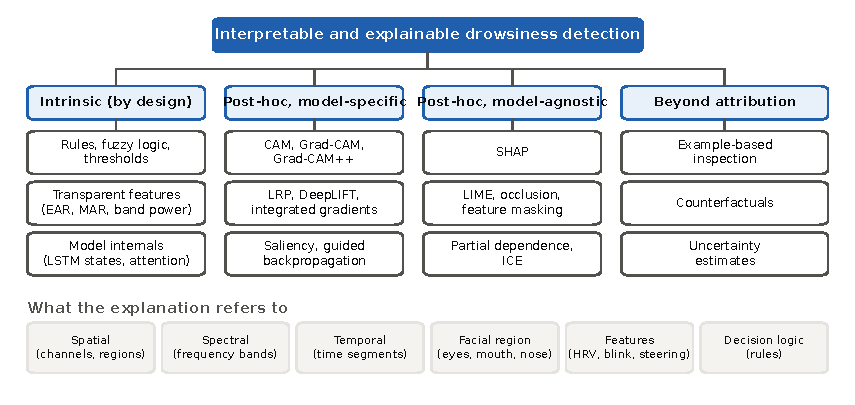
\includegraphics[width=\textwidth]{fig1_taxonomy}
\caption{Taxonomy used in this review. The upper part groups methods by how the explanation is produced; the lower band lists what an explanation can refer to. EAR: eye aspect ratio; MAR: mouth aspect ratio; ICE: individual conditional expectation.}
\label{fig:taxonomy}
\end{figure*}

\subsection{Intrinsic methods}
\textit{Rules and logic.} Rule-based systems make every decision traceable. Beles \textit{et al.}~\cite{beles2024driver} fuse physiological and camera cues with fuzzy rules, and Ersoy \textit{et al.}~\cite{ersoy2026improving} calibrate eye and mouth thresholds to each driver. Fuzzy systems range widely in how readable they are. Gao \textit{et al.}~\cite{gao2025comprehensive} stack Takagi--Sugeno--Kang classifiers whose rules use linguistic levels but refer to features only by index, whereas Hu \textit{et al.}~\cite{hu2026human} and Yan and Xie~\cite{yan2026toward} write interval type-2 rules over named eye and mouth measures, the latter constraining the membership functions so that the sets stay ordered and distinguishable. Georgiadis \textit{et al.}~\cite{georgiadis2026timeaware} go furthest towards symbolic reasoning, with an ontology whose logic rules map physiological thresholds to driver states.

\textit{Transparent features.} Albadawi \textit{et al.}~\cite{albadawi2023realtime} feed eye aspect ratio, mouth aspect ratio and head position to simple classifiers, so an alarm can be traced to a named cue.

\textit{Model internals.} Other studies read explanations from LSTM hidden states \cite{cui2021subject}, attention scores \cite{an2024attention,gao2024sftnet} or the eigenvalues of a recurrent weight matrix \cite{gao2025idsrn}. Internal states are built in, but that does not establish that they explain the decision. Attention weights in particular need not track input importance \cite{jain2019attention}, and Section~\ref{sec:attention} shows that the question is live in this domain.

\subsection{Post-hoc, model-specific methods}
Class activation mapping (CAM) \cite{zhou2016cam} weights the last convolutional feature maps by the class weights of a global-average-pooling network. Grad-CAM \cite{selvaraju2017gradcam} extends the idea to other architectures using gradients, Grad-CAM++ \cite{chattopadhay2018gradcampp} uses higher-order gradient terms, and LayerCAM \cite{jiang2021layercam} weights each location by its positive gradients and works at any layer. This family dominates the vision studies. Layer-wise relevance propagation (LRP) \cite{bach2015lrp} passes the output score backwards layer by layer, and integrated gradients \cite{sundararajan2017axiomatic} accumulate gradients along a path from a baseline to the input. These produce finer-grained maps, and the integrated-gradients result depends on the chosen baseline. Attention rollout \cite{abnar2020quantifying} combines attention across transformer layers and needs the same testing as other attention maps; one reviewed study applies it across modalities \cite{theivadas2025dynamic}.

\subsection{Post-hoc, model-agnostic methods}
SHAP \cite{lundberg2017shap} assigns each feature a Shapley value and, in the studies reviewed, is applied mostly to tree models on hand-crafted features. LIME \cite{ribeiro2016lime} fits a simple local surrogate, and occlusion \cite{zeiler2014visualizing} measures the score drop when part of the input is hidden. PGM-Explainer perturbs graph nodes and fits a Bayesian network over them; it appears here in one study on a graph network \cite{zeynalpour2025multimethod}. Partial dependence \cite{friedman2001greedy} and individual conditional expectation plots \cite{goldstein2015ice} show how predictions change with a feature, but they assume the feature varies independently of the others, which is doubtful for correlated physiological measures.

\subsection{Beyond attribution}
Three other forms appear rarely. McDonald \textit{et al.}~\cite{mcdonald2014steering} explain a model by inspecting example inputs from each cell of the confusion matrix. Counterfactual explanations \cite{wachter2017counterfactual}, the smallest change that would flip a decision, have been proposed for drowsiness alarms \cite{jha2025realtime} but not evaluated. Uncertainty estimates \cite{oise2026enhancing} complement an explanation but do not attribute a decision.

\begin{table}[!t]
\centering
\caption{Placement of the Reviewed Studies in the Taxonomy}
\label{tab:taxonomy}
\footnotesize
\begin{tabularx}{\columnwidth}{@{}L{0.33\columnwidth}Y@{}}
\toprule
\textbf{Method family} & \textbf{Studies} \\
\midrule
\multicolumn{2}{@{}l}{\textit{Intrinsic}} \\
Rules, fuzzy logic & \cite{beles2024driver,ersoy2026improving,gao2025comprehensive,hu2026human,yan2026toward} \\
Ontology, logic rules & \cite{georgiadis2026timeaware} \\
Transparent features & \cite{albadawi2023realtime} \\
Model internals & \cite{cui2021subject,an2024attention,gao2025idsrn,gao2024sftnet} \\
\midrule
\multicolumn{2}{@{}l}{\textit{Post-hoc, model-specific}} \\
CAM family & \cite{cui2022eeg,cui2022compact,feng2025id3rsnet,wu2024driver,saxena2026lowlight,rafy2026domain,oise2026enhancing,nomura2025drowsiness,florez2023cnn,hassan2025realtime,zeynalpour2025multimethod,jewel2025lightweight,sasikala2026robust,nayomi2026vision} \\
LRP, integrated gradients & \cite{seo2025driver,saxena2026lowlight} \\
Feature-map visualisation & \cite{xu2026dynamic} \\
\midrule
\multicolumn{2}{@{}l}{\textit{Post-hoc, model-agnostic}} \\
SHAP & \cite{hasan2024validation,vitorino2023adversarial,puspasari2026predicting,zhou2021predicting,jha2025realtime,zhu2025madfm,guan2025fatigue,zeynalpour2025multimethod} \\
LIME, occlusion & \cite{saxena2026lowlight,zeynalpour2025multimethod} \\
PGM-Explainer & \cite{zeynalpour2025multimethod} \\
Partial dependence, ICE & \cite{hasan2024validation} \\
\midrule
\multicolumn{2}{@{}l}{\textit{Combined}} \\
Selection pipeline + SHAP & \cite{jiang2026eeg} \\
Kernel weights + masking & \cite{zhou2026sedriven} \\
Rule + Grad-CAM & \cite{florez2024realtime} \\
Graph attention + occlusion & \cite{zhuang2024connectivity} \\
Modality attention + saliency & \cite{theivadas2025dynamic} \\
\midrule
\multicolumn{2}{@{}l}{\textit{Other}} \\
Example inspection & \cite{mcdonald2014steering} \\
Band correlation, t-SNE & \cite{zhang2024multimodal} \\
Counterfactuals & \cite{jha2025realtime} \\
Uncertainty & \cite{oise2026enhancing} \\
Claimed, none shown & \cite{alarnaout2025exploiting} \\
\bottomrule
\end{tabularx}
\end{table}

\section{Explanations by Modality}
\label{sec:modalities}

Tables~\ref{tab:eeg}--\ref{tab:vision} summarise each study. The last column gives the four appraisal ratings: P, explanation agrees with known physiology; E, explanation evaluated; S, tested on unseen drivers; C, code public.

\subsection{EEG and EOG}
EEG holds the richest explanation work, and one pattern runs through it: the two classes are explained by different kinds of evidence. From inspecting selected samples, Cui \textit{et al.} read drowsy decisions as resting on theta bursts and alpha spindles, which match the literature, and alert decisions as resting largely on muscle activity at peripheral channels, eye movements and slow sensor drift \cite{cui2022eeg,cui2022compact,cui2021subject}. ID3RSNet shows the same split, although its explanations rely less on single blink-like peaks than an earlier compact model \cite{feng2025id3rsnet}. The authors of these studies treat this as a finding and suggest that artefact handling should be a deliberate design choice. If correct, it is also a warning, because artefacts that help on one recording setup may not transfer to other hardware. Section~\ref{sec:casestudy} tests this reading across all windows: support is weak on the 11-subject subset and clearer on all 27 subjects.

Zhuang \textit{et al.}~\cite{zhuang2024connectivity} reach a similar result on the same data with a different model and a different explanation method. In a graph network with a learned connectivity matrix, occlusion maps highlighted alpha spindles in correctly classified drowsy samples for 10 of 11 subjects and beta oscillations in alert samples for all 11, and highlighted segments had significantly higher alpha power when the model predicted drowsy. This is the strongest corroboration of the drowsy reading in the set. The maps themselves were inspected on examples, however, and the learned ``connectivity'' is a weighting inside the model, so its reduction in occipital and parietal regions describes the network at least as much as the brain.

Seo \textit{et al.}~\cite{seo2025driver}, who removed eye and muscle artefacts with independent component analysis, obtained cortical explanations: LRP on source-space band power highlighted frontal theta and parieto-occipital alpha, and group statistics confirmed the alpha increase. Their model reached 96.9\% after fine-tuning on each driver but stayed near chance (50.8\%) on unseen drivers. Plausible explanations and cross-subject generalisation are therefore separate properties.

Other studies complicate the theta and alpha story. An \textit{et al.}~\cite{an2024attention} read band importance from attention scores: theta and alpha exceeded beta for the three best-predicted subjects, but not consistently for the three worst, and no other subjects were analysed. Jiang \textit{et al.}~\cite{jiang2026eeg} used a transparent selection pipeline, nested inside leave-one-subject-out folds, and found eight features selected in every fold. These were amplitude statistics plus beta and gamma power; theta and alpha power were not retained. The labels were task stages in a laboratory task, so a stable feature may track time on task rather than fatigue. Zhou \textit{et al.}~\cite{zhou2026sedriven} applied no formal XAI method but probed the model through band masking and channel removal; theta and alpha were the strongest narrow bands, although every single band still gave 83--92\%. Gao \textit{et al.}~\cite{gao2024sftnet} found gamma the most active band under attention and the best with beta when trained alone. Gamma at temporal sites is where muscle contamination is expected, and the paper does not discuss this possibility, so a physiological reading of the band remains open.

Explanations can also claim more than the montage allows. Xu \textit{et al.}~\cite{xu2026dynamic} read activation maps from SEED-VIG as evidence about dorsolateral prefrontal cortex, the precuneus and the posterior cingulate, but SEED-VIG records only 17 temporal and posterior scalp channels \cite{zheng2017multimodal}, and the maps are shown for three chosen subjects. Gao \textit{et al.}~\cite{gao2025idsrn} state that recurrent-matrix poles reveal 6~Hz theta activity, but they report no pole values, and the recurrence runs over 8-s feature windows rather than raw samples, which makes that reading hard to reconcile. Wu \textit{et al.}~\cite{wu2024driver} use EEG to study hand--foot coordination under fatigue, and LayerCAM on connectivity matrices agrees with their graph statistics on frontal and central connections. Their study shows XAI used for scientific exploration, but a CNN treats adjacent matrix cells as neighbours, and those cells are neighbours only through channel ordering, so regions in the map may depend on that ordering. Their test split is also random over overlapping windows.

Interpretable fuzzy models can also fall short of being readable. Gao \textit{et al.}~\cite{gao2025comprehensive} conclude that their stacked classifier has good interpretability from example rules such as ``the 26th feature is high'', but the rules are never mapped to channels, bands or any physiological claim, so a reader cannot check them. Precision, recall and F1 are also identical within every row of both of its results tables, which should be clarified before the numbers are compared.

Explanations also help audit data. Cui \textit{et al.} traced errors to sensor noise and to alert-labelled samples full of alpha spindles, which suggests label noise in reaction-time labels \cite{cui2022eeg,cui2022compact}. Zhuang \textit{et al.} similarly link errors to samples where spindles and beta activity co-exist \cite{zhuang2024connectivity}.

\begin{table*}[!t]
\centering
\caption{EEG and EOG Studies. Ratings P/E/S/C: Y yes; P partly; N no or not shown; F faithfulness tested; p partial check only; s stated, not verifiable; -- not applicable. LOSO: Leave-One-Subject-Out; RT: Reaction Time}
\label{tab:eeg}
\scriptsize
\setlength{\tabcolsep}{3pt}
\begin{tabularx}{\textwidth}{@{}L{1.5cm}L{2.7cm}L{2.3cm}L{2.2cm}YL{3.1cm}L{0.95cm}@{}}
\toprule
\textbf{Study} & \textbf{Data; labels} & \textbf{Model} & \textbf{Explanation} & \textbf{What it showed} & \textbf{Result (test scheme)} & \textbf{P/E/S/C} \\
\midrule
Cui 2023 \cite{cui2022eeg} & Cao subset, 11 subj.; RT & InterpretableCNN, 30 channels & CAM + CNN-Fixation (post-hoc) & Drowsy: theta bursts, alpha spindles, central sites. Alert: EMG at peripheral channels, eye activity & 78.35\% balanced, 77.70\% unbalanced (LOSO) & P/N/Y/Y \\
Cui 2022 \cite{cui2022compact} & Cao subset, 11 subj.; RT & Compact CNN, Oz only & CAM (post-hoc) & Drowsy: alpha spindles, theta--delta bursts. Alert: EMG, sensor drift. Exposes probable mislabelled samples & 73.22\% balanced (LOSO) & P/N/Y/Y \\
Cui 2021 \cite{cui2021subject} & Cao subset, 11 subj.; RT & CNN-LSTM, Oz only & LSTM hidden states (intrinsic) & Decision builds over time; alpha spindles for drowsy, EMG and drift for alert & 72.97\% balanced (LOSO) & P/N/Y/Y \\
Feng 2025 \cite{feng2025id3rsnet} & Cao subset, 11 subj.; RT & ID3RSNet, Oz only & EEG CAM (post-hoc) & Same split; more spindle regions and fewer single blink-like peaks than the compact CNN & 77.16\% balanced, 74.72\% unbalanced (LOSO) & P/F/Y/N \\
Zhuang 2024 \cite{zhuang2024connectivity} & Cao subset, 11 subj.; RT & Connectivity-aware graph network, 30 channels & Band attention, learned graphs, occlusion (combined) & Theta leads attention and single-band retraining; occlusion finds alpha spindles for drowsy, beta for alert & 70.5\% all bands, 72.6\% theta only (LOSO) & Y/p/Y/Y \\
Seo 2025 \cite{seo2025driver} & Private, 21 subj.; video-rated KSS & 3D CNN on source-space band power & LRP (post-hoc) & Frontal theta, parieto-occipital alpha; alpha confirmed by group statistics & 96.9\% within-subject; 50.8\% on unseen drivers & Y/N/N/N \\
An 2024 \cite{an2024attention} & Cao, 27 subj.; RT regression & ACF-GCN & Attention scores (intrinsic) & Theta, alpha above beta in three best subjects; mixed in three worst & RMSE 0.788 s, $r = 0.313$ (LOSO) & P/N/Y/N \\
Jiang 2026 \cite{jiang2026eeg} & Private, 16 subj., lab task; task stage & EfficientLSTM, 3 classes & Feature selection + SHAP (combined) & Stable features: amplitude statistics, beta, gamma; theta and alpha not retained & 74.54\% (nested LOSO) & N/p/Y/N \\
Zhou 2026 \cite{zhou2026sedriven} & SEED-VIG, 21 subj., PERCLOS; Cao subset, RT & DCAMNet & Kernel weights, band masking, channel removal (combined) & Theta and alpha strongest narrow bands; all bands 83--92\% & 85.43\% SEED-VIG, 79\% Cao (LOSO); 97.47\% mixed & P/N/Y/N \\
Gao 2024 \cite{gao2024sftnet} & SEED-VIG, 23 subj.; PERCLOS & Attention, separable convolution, LSTM & Spatial, frequency attention (intrinsic); single-band training & Gamma most active; delta high under attention but last when trained alone & 87.13\% five-fold; 85.3\% (LOSO) & P/p/Y/Y \\
Xu 2026 \cite{xu2026dynamic} & SEED-VIG, 23 subj.; PERCLOS, 3 classes & Dynamic topology graph network & Activation maps, three subjects (post-hoc) & Read as prefrontal and default-mode effects; montage has temporal and posterior sites only & 89.1\% within-subject; LOSO described, no separate result found & P/N/s/N \\
Wu 2024 \cite{wu2024driver} & Private, 30 subj.; KSS, 3 levels & ResNet18 on PLI connectivity matrices & LayerCAM (post-hoc) & Frontal, central connections; agrees with graph statistics; depends on channel order & 94.1\% (random 90/10 of overlapping windows) & P/N/N/N \\
Gao 2025a \cite{gao2025comprehensive} & Private, 14 subj.; SEED-VIG, 14 subj., PERCLOS & Stacked TSK fuzzy classifier & Fuzzy rules (intrinsic) & Rules over unnamed feature indices; not linked to channels or bands & 83.84\%, 80.06\% (random 80/20, five-fold) & N/N/N/N \\
Gao 2025b \cite{gao2025idsrn} & SEED-VIG; PERCLOS & IDSRN polynomial recurrent & Recurrent poles (intrinsic) & States a 6 Hz theta pole; values not shown & 97.06\% (pooled 10-fold) & N/N/N/N \\
\midrule
Cui 2023 \cite{cui2023towards}$^{\dagger}$ & Three EEG datasets, incl. Cao subset & EEGNet, InterpretableCNN & Seven attribution methods compared & Gradient$\times$input, DeepLIFT, integrated gradients, LRP beat random maps; saliency, deconvolution, guided backpropagation mostly do not & Methods study (LOSO on drowsiness data) & Y/F/Y/Y \\
\bottomrule
\multicolumn{7}{@{}l}{$^{\dagger}$Methods study, excluded from the appraisal counts.}
\end{tabularx}
\end{table*}

\subsection{ECG and HRV}
Explanation work on cardiac signals consists almost entirely of SHAP on classical models over hand-crafted HRV features. We found no ECG drowsiness model explained by attribution on the raw signal. Vitorino \textit{et al.}~\cite{vitorino2023adversarial} ranked SD2/SD1, a nonlinear HRV measure, as the most consistently important feature, and showed that plausible adversarial perturbations of HRV features sharply degrade most models. They tested the robustness of predictions, not of explanations, which remains open.

Puspasari \textit{et al.}~\cite{puspasari2026predicting} used subject-grouped validation and report SHAP rankings led by mean RR interval and mean heart rate. Their summary plot illustrates a problem with redundant inputs. The two features are mathematical inverses, yet high values of both push the prediction away from the late-session class, assuming the plotted values refer to that class. High RMSSD also pushes towards it, against the text's account of reduced HRV. Correlated features can thus produce rankings that are hard to read physiologically. In addition, the label is session order, so the explanation describes time on task as much as fatigue.

AlArnaout \textit{et al.}~\cite{alarnaout2025exploiting} describe their tree models as easy to interpret but show no explanation. They also label windows from heart-rate thresholds while mean RR is an input feature, although the paper states that labels and inputs are independent.

\begin{table*}[!t]
\centering
\caption{ECG/HRV, Vehicle-Based, Multimodal and Knowledge-Based Studies. Ratings as in Table~\ref{tab:eeg}}
\label{tab:cardiac}
\scriptsize
\setlength{\tabcolsep}{3pt}
\begin{tabularx}{\textwidth}{@{}L{1.7cm}L{2.7cm}L{2.2cm}L{2.2cm}YL{3cm}L{1.05cm}@{}}
\toprule
\textbf{Study} & \textbf{Signals; data; labels} & \textbf{Model} & \textbf{Explanation} & \textbf{What it showed} & \textbf{Result (test scheme)} & \textbf{P/E/S/C} \\
\midrule
Vitorino 2023 \cite{vitorino2023adversarial} & HRV; DROZY, 14 subj.; PVT & SVM, KNN, XGBoost, LightGBM & SHAP & SD2/SD1 most consistent; top 18 features match the full set's F1 & Macro-F1 81.58\% (random split of overlapping windows) & N/p/N/N \\
Puspasari 2026 \cite{puspasari2026predicting} & HRV; private, 40 subj.; session order or sleep condition & XGBoost, RF, LR & SHAP & Mean RR, mean HR, LF lead; redundant features with conflicting directions & 77.0\%, AUC 0.785 (grouped 5-fold) & Y/p/Y/N \\
AlArnaout 2025 \cite{alarnaout2025exploiting} & PPG-HRV; 10 subj. + 3 drivers; heart-rate rule & Six classifiers, RF best & Claimed, none shown & No explanation output & 86.05\% (window-level 4-fold) & N/N/N/N \\
McDonald 2014 \cite{mcdonald2014steering} & Steering angle; NADS simulator, 72 drivers; observer rating & Random forest & Example traces & ``Steering holds'' read as drowsy; authors state the features used are unclear & Accuracy 0.79, AUC 0.70 (10-fold, not by driver) & Y/N/N/N \\
Zhu 2025 \cite{zhu2025madfm} & Steering, lateral motion; simulator, 25 male students; KSS, 3 levels & Random forest + mRMR and SHAP selection & SHAP & Steering-angle SD, lateral acceleration rise with severe fatigue; mild class least separable & 93.71\% (window-level five-fold and 7:3 split) & Y/p/N/N \\
Zhou 2021 \cite{zhou2021predicting} & Heart, breathing, steering; simulator, 20 subj.; PERCLOS & XGBoost regression & SHAP (global, local) & Heart rate and breathing lead; steering matters less & Adj.\ $R^2$ 0.996 (random 10-fold over 1-s samples) & Y/p/N/N \\
Guan 2025 \cite{guan2025fatigue} & HRV, EDA, wrist motion, vehicle; simulator, 33 drivers; timed session & XGBoost, 3 states & SHAP & Wrist motion and vehicle dynamics lead; HRV and EDA lower & 94.28\% (23 train, 10 unseen drivers) & P/N/Y/N \\
Hasan 2024 \cite{hasan2024validation} & EEG, EOG, ECG; lab vigilance task, 26 subj.; KSS & KNN, SVM, RF & SHAP, partial dependence & Blink duration, AVR, central theta, occipital alpha lead; HRV low; methods agree ($r = 0.849$) & 80.1\% (leave-one-participant-out) & Y/p/Y/N \\
Zhang 2024 \cite{zhang2024multimodal} & EEG, EOG; SEED-VIG, 21 subj.; PERCLOS & CNN + transformer fusion & Band correlation, t-SNE & Theta, alpha correlate best; modality contribution not attributed & $r = 0.887$ (LOSO) & Y/N/Y/N \\
Theivadas 2025 \cite{theivadas2025dynamic} & EEG, ECG, face, steering; DROZY, NTHU-DDD, ``SIM-DROWSY'' & Gated cross-attention transformer & Attention rollout + saliency (combined) & Behavioural attention when alert, physiological rising at onset, in one example & 89.7\% balanced on DROZY (LOSO stated); not verifiable & N/p/s/N \\
Beles 2024 \cite{beles2024driver} & EOG/EEG, eye images; lab and road, apparently one driver & ANN + fuzzy fusion & Fuzzy rules (intrinsic) & Decision logic readable; dominant input not analysed & No system-level evaluation & Y/N/N/N \\
Jha 2025 \cite{jha2025realtime} & Eye, head, steering; data not named & Described only & SHAP, counterfactuals & No concrete output reported & Claims without supporting data & N/N/N/N \\
Georgiadis 2026 \cite{georgiadis2026timeaware} & HR, HRV, respiration, SpO2; pilot + TimeGAN synthetic data & OWL ontology, logic rules & Rules (intrinsic) & Every inference traceable; correctness against driver state not tested & No detection result (logical consistency only) & Y/N/--/N \\
\midrule
Askari 2026 \cite{askari2026physiologically}$^{\dagger}$ & EEG, EMG, GSR; MPDB, 30 subj.; manoeuvre & XGBoost + LightGBM & SHAP & Used to argue plausibility; EEG share of SHAP partly reflects feature count & 80.91\% (random window split) & Y/N/N/N \\
\bottomrule
\multicolumn{7}{@{}l}{$^{\dagger}$Classifies manoeuvres, not drowsiness; excluded from the appraisal counts. Zhou 2021 and Askari 2026 are preprints.}
\end{tabularx}
\end{table*}

\subsection{Vision}
\label{sec:vision}
Vision studies mostly show Grad-CAM heatmaps of eyes and mouth, and the usual evidence is a few images judged by eye. Saxena \textit{et al.}~\cite{saxena2026lowlight} apply five methods to one model and report how well the maps overlap detected eye and mouth regions, which measures plausibility; their limitations section acknowledges that the explanations were evaluated only qualitatively, with no faithfulness assessment. Rafy \textit{et al.}~\cite{rafy2026domain} give the most instructive result among the heatmap studies: maps on the realistic UTA-RLDD data partly fall on background regions, and focus metrics drop as recording conditions become less controlled, so the explanation exposes a dataset effect that accuracy conceals. Oise \textit{et al.}~\cite{oise2026enhancing} name Grad-CAM++ and uncertainty as ensuring transparency, but the paper contains no explanation output, and its figures do not match its headline metrics. Jewel \textit{et al.}~\cite{jewel2025lightweight} report eyelid and pupil maps as fostering trust without analysing them, and their 99.28\% on UTA-RLDD follows image shuffling that they describe as preventing subject bias, although shuffling before a split places frames of one person on both sides of it.

Zeynalpour \textit{et al.}~\cite{zeynalpour2025multimethod} stand apart. They apply SHAP, occlusion, PGM-Explainer and Grad-CAM to a graph network over body and face keypoints and score each with fidelity measures across sparsity levels. The methods agree that facial keypoints, especially the eyes, drive not-alert predictions, but disagree on alert ones: SHAP and PGM-Explainer favour hands and upper body, occlusion mostly the face, and Grad-CAM spreads across both. Section~\ref{sec:attention} returns to the fidelity scores. The setting is limited, with train-driver states acted at a desk and two test participants, so hand movement may reflect instructions to mimic driving rather than alertness, and the study does not report the model's accuracy.

Florez \textit{et al.}~\cite{florez2023cnn,florez2024realtime} use Grad-CAM on a handful of images to choose between networks of almost equal accuracy, even though many maps fall on the nose, cheek or forehead. Explanations here steer model selection without having been tested. Nomura \textit{et al.}~\cite{nomura2025drowsiness} use near-infrared face images and find activation mainly around the eyes, with additional responses along the nose, mouth and forehead, which they link to blood-flow changes. They note that eye activation may reflect blinking; masking the eyes would test this, but was not done.

A subtler issue is that many vision labels are really eye-state labels. When the class is simply open versus closed, as in Hassan \textit{et al.}~\cite{hassan2025realtime} and the Florez studies, a heatmap on the eyelid confirms the label definition and says little about drowsiness. Rule-based alternatives avoid opacity \cite{albadawi2023realtime,ersoy2026improving}, and personalising thresholds narrowed part of the gap to a CNN in one preprint \cite{ersoy2026improving}, but these too need independent labels. In the study of Albadawi \textit{et al.}, the labels are generated from thresholds on the same features the classifier receives.

Two further rule systems feed a controller. Hu \textit{et al.}~\cite{hu2026human} and Yan and Xie~\cite{yan2026toward} turn eye and mouth openness into a fatigue level through interval type-2 fuzzy rules and use that level to set steering authority. Their rules are the most readable in the set, and they report control gains with three simulator drivers, but neither checks the fatigue estimate against any independent measure of drowsiness.

Finally, two conference papers with different author lists \cite{sasikala2026robust,nayomi2026vision} report identical results tables at all three train--test ratios, with a maximum of 98.87\%, share long runs of text and equations, and name no dataset, subject count or labelling procedure. We count them as one study, rate that study on what is reported, and do not rely on its numbers.

\begin{table*}[!t]
\centering
\caption{Vision Studies. Ratings as in Table~\ref{tab:eeg}}
\label{tab:vision}
\scriptsize
\setlength{\tabcolsep}{3pt}
\begin{tabularx}{\textwidth}{@{}L{1.6cm}L{2.8cm}L{2.3cm}L{2.1cm}YL{3cm}L{1.15cm}@{}}
\toprule
\textbf{Study} & \textbf{Data; labels} & \textbf{Model} & \textbf{Explanation} & \textbf{What it showed} & \textbf{Result (test scheme)} & \textbf{P/E/S/C} \\
\midrule
Saxena 2026 \cite{saxena2026lowlight} & Six public datasets; dataset labels mapped to three classes & InceptionV3 + dual attention & Grad-CAM, IG, LRP, occlusion, LIME & Authors report eyes and mouth; localisation scores for all methods, no faithfulness test & 96.2--98.5\% per dataset (subject split stated) & Y/p/s/N \\
Rafy 2026 \cite{rafy2026domain} & MRL Eye, NTHU-DDD, UTA-RLDD; dataset labels & Swin-based ViT & Grad-CAM & Periocular focus; background attention on UTA-RLDD; IoU above 0.71 with annotations & 97.2--98.7\% random split; 92--94.5\% cross-dataset & P/p/s/N \\
Oise 2026 \cite{oise2026enhancing} & Six datasets; mixed labelling & MobileNetV2 + ViT & Grad-CAM++, MC dropout & Described in text only; no map shown & 99.27\% claimed; figures disagree & N/N/s/N \\
Zeynalpour 2025 \cite{zeynalpour2025multimethod} & Body, face keypoints; private, 20 subj.; acted states, train-driver setting & Directed graph network & SHAP, occlusion, PGM-Explainer, Grad-CAM & Eyes for not alert; explainers differ for alert. SHAP best Fidelity+, PGM-Explainer best Fidelity$-$ & Accuracy not reported (18 train, 2 test) & Y/F/Y/N \\
Nomura 2025 \cite{nomura2025drowsiness} & Private NIR, 10 subj.; observer rating & Small CNN & Grad-CAM & Mainly around the eyes, also nose, mouth, forehead & 90.7\% $\pm$ 16.9, worst subject 47.3\% (LOSO) & P/N/Y/N \\
Jewel 2025 \cite{jewel2025lightweight} & MRL Eye, UTA-RLDD; dataset labels & CoAtNet variant & Grad-CAM & Eyelids, pupils; no analysis of the maps & 99.28\% UTA-RLDD, 98.81\% MRL (shuffled image split) & P/N/N/N \\
Florez 2023 \cite{florez2023cnn} & NITYMED, 6 videos; eye state & Three CNN backbones & Grad-CAM & Used to choose a model; many maps off the eyes & 99.71\% (random frame split) & P/N/N/N \\
Florez 2024 \cite{florez2024realtime} & NITYMED, 6 videos; eye state & DD-AI CNN + MAR rule & Grad-CAM + rule (combined) & Proposed CNN on the eyes in five images; yawn rule transparent & 99.88\% frame split; 96.55\% in-car demo & P/N/N/N \\
Hassan 2025 \cite{hassan2025realtime} & MRL Eye, NTHU-DDD, CEW; eye state & ViT, Swin, CNNs & CAM on two images & Eyelid or eye area, which is what the label defines & 99.15\% (random image split) & P/N/N/N \\
Sasikala 2026, Nayomi 2026 \cite{sasikala2026robust,nayomi2026vision} & Unnamed infrared images; subjects, labels not stated & Eye detector + attention CNN & CAM, Grad-CAM & Eye region, described only & 98.87\% (ratio split, grouping not stated) & N/N/N/N \\
Albadawi 2023 \cite{albadawi2023realtime} & NTHU-DDD, 23 subj.; threshold-generated & RF, NN, SVM on EAR, MAR, head pose & Transparent features (intrinsic) & Alarm traceable to eyes, yawn, nod; importance not measured & 99\% (random 70/30 after oversampling) & Y/N/N/N \\
Ersoy 2026 \cite{ersoy2026improving} & MRL Eye, Yawn, custom; eye, yawn state & Personal thresholds vs CNN & Rules (intrinsic) & Personal thresholds raise accuracy, remain readable & Eye state 93.2\% rules, 99.1\% CNN (random split) & Y/N/N/N \\
Hu 2026 \cite{hu2026human} & Facial landmarks; simulator, 3 drivers; no drowsiness label & IT2 fuzzy rules + shared-steering controller & Rules (intrinsic) & Eye and mouth rules; estimate not validated & Control metrics only & Y/N/--/N \\
Yan 2026 \cite{yan2026toward} & Facial landmarks; simulator, 3 drivers; no drowsiness label & Constrained IT2 fuzzy rules + controller & Rules (intrinsic) & Ordered, distinguishable sets; estimate not validated & Control metrics only & Y/N/--/N \\
\midrule
Ghoddoosian 2019 \cite{ghoddoosian2019realistic}$^{\dagger}$ & UTA-RLDD, 60 subj.; KSS self-report & Blink features + HM-LSTM & None & Alert and drowsy separable; humans reach 57.8\% & 65.2\% video-level (subject-independent 5-fold) & --/N/Y/Y \\
\bottomrule
\multicolumn{7}{@{}l}{$^{\dagger}$Dataset paper with no explanation method; a baseline for comparison, excluded from the appraisal counts. Ersoy 2026 is a preprint.}
\end{tabularx}
\end{table*}

\subsection{Vehicle-based signals}
Vehicle signals remain the least explored. McDonald \textit{et al.}~\cite{mcdonald2014steering} explain a steering-based random forest by inspecting example traces: low-variability ``steering holds'' count as drowsy, and ordinary low-activity driving causes false alarms. The authors acknowledge that it is unclear which features the forest uses, and variable importance was not reported. Zhu \textit{et al.}~\cite{zhu2025madfm} give the clearest vehicle-only explanation in the set. SHAP on a steering-signal random forest shows steering-angle variability and lateral acceleration rising with severe fatigue, while feature values near their medians point to mild fatigue, the class most often confused. That account of where the method is weak is useful, but SHAP is also used to select the features, the paper describes no nesting of selection inside folds, and windows are not grouped by driver, so the 93.71\% is likely optimistic. The sample is also all male students. Zhou \textit{et al.}~\cite{zhou2021predicting} include steering among SHAP-ranked features, where it ranks below heart and breathing measures, although random splitting of one-second samples makes their accuracy hard to interpret. We found no vehicle-only deep model with formal attribution in our set.

\subsection{Multimodal fusion}
Fusion raises a question that single-signal work does not: how much does each modality contribute? The studies here rarely answer it. Hasan \textit{et al.}~\cite{hasan2024validation} come closest among the verifiable studies, finding that blink features and central theta outrank HRV under SHAP and partial dependence, and they report the strongest validation in this group, comparing six schemes on the same data and arguing that leave-one-participant-out gives the most general results. Zhang \textit{et al.}~\cite{zhang2024multimodal} interpret a deep EEG--EOG model through band correlations and t-SNE but do not attribute the fused prediction; because EOG measures blinks directly and the label is eye-tracker PERCLOS, the EOG branch may sit close to the label itself. Summing SHAP values by modality is also misleading when modalities differ in feature count, as Askari \textit{et al.}~\cite{askari2026physiologically} partly concede.

Guan \textit{et al.}~\cite{guan2025fatigue} hold out ten unseen drivers and reach 94.28\% across normal, distracted and fatigued states, and SHAP ranks wrist-motion and vehicle-dynamics features above HRV and skin conductance. Here the explanation is most useful as a warning. Each state was a separate timed session, with a movie on a tablet in the distraction session and a set speed range in the fatigue session, so the leading features may separate the task in each session rather than the driver's internal state. The authors also describe SHAP as yielding a causal feature weighting and name DeepExplainer for a tree ensemble; SHAP is not causal, and TreeExplainer would be the expected choice.

Theivadas and Ponnan~\cite{theivadas2025dynamic} present a design aimed directly at the modality question: a dashboard of attention over time, in which behavioural cues dominate when alert and physiological cues rise at drowsiness onset. We cite this as a design idea and cannot verify its results. Its top physiological features include skin-conductance level, which none of its three described datasets is said to record; we could not locate a source for ``SIM-DROWSY'', whose citation number falls beyond the printed reference list; and the ``expert annotations'' behind its consistency score are not described. Beles \textit{et al.}~\cite{beles2024driver} offer readable rules but no quantitative test on synchronised data, and Jha \textit{et al.}~\cite{jha2025realtime} propose counterfactual advice without reported data.

\subsection{Knowledge-based reasoning}
Georgiadis \textit{et al.}~\cite{georgiadis2026timeaware} take the opposite position from the black-box models. An ontology with logic rules classifies heart rate, HRV, respiration and SpO2 into threshold categories personalised by age and sex and infers states such as drowsiness suspected, so every inference can be traced to explicit rules. Its evaluation covers logical consistency and competency questions on pilot data augmented with synthetic series, and the authors say plainly that this is neither a real-world benchmark nor clinically definitive. Drowsiness level is also an input from elsewhere, so the system explains how evidence is combined, not how drowsiness is detected. Together with the fuzzy controllers above \cite{hu2026human,yan2026toward}, it marks one end of a trade-off in the reviewed set: full transparency with no evidence of correct detection.

\section{Datasets}
\label{sec:datasets}

Table~\ref{tab:datasets} lists the public datasets used by the reviewed studies. Two features matter for explanation. First, the evidence base is narrow. Seven of the ten EEG papers use the Cao \textit{et al.} lane-departure dataset \cite{cao2019multichannel}, and six use the same 11-subject subset, so claims about what EEG models learn rest largely on one simulator, one labelling rule and about eleven drivers. Second, datasets differ in what their labels mean: reaction time, PERCLOS, self-report, observer rating or eye state. An explanation can only be as meaningful as the label it explains. MRL Eye and CEW, for instance, record whether the eye is open and do not measure drowsiness at all.

Several studies also use private data \cite{seo2025driver,jiang2026eeg,hasan2024validation,puspasari2026predicting,nomura2025drowsiness,zhou2021predicting}, which prevents independent checks of their explanations.

\begin{table*}[!t]
\centering
\caption{Public Datasets Used by the Reviewed Studies}
\label{tab:datasets}
\scriptsize
\setlength{\tabcolsep}{3pt}
\begin{tabularx}{\textwidth}{@{}L{2.5cm}L{1.6cm}L{4cm}L{3.1cm}Y@{}}
\toprule
\textbf{Dataset} & \textbf{Subjects} & \textbf{Setting} & \textbf{Signals} & \textbf{Labels} \\
\midrule
Cao \textit{et al.} \cite{cao2019multichannel} & 27 (62 sessions) & 90-min night-time VR lane keeping & 30-channel EEG, 500 Hz & Reaction time to lane departures \\
SEED-VIG \cite{zheng2017multimodal} & 23 & About 2 h simulated highway driving & 17-channel EEG, forehead EOG, 200 Hz & PERCLOS from eye-tracking glasses (binarised differently across studies) \\
DROZY \cite{massoz2016drozy} & 14 & Three sessions with rising sleep deprivation; vigilance test & EEG, EOG, ECG, EMG, near-infrared video & KSS and vigilance-test reaction time \\
NTHU-DDD \cite{weng2017nthu} & 36 & Simulated driving, acted drowsiness; day and night, glasses & Infrared video & Drowsy and non-drowsy behaviours \\
UTA-RLDD \cite{ghoddoosian2019realistic} & 60 & Self-recorded indoors, not driving, about 30 h & RGB phone or webcam video & KSS self-report, three classes \\
MRL Eye \cite{fusek2018mrl} & 37 & Infrared eye crops & About 85{,}000 images & Eye open or closed \\
YawDD \cite{abtahi2014yawdd} & Not stated here & Drivers in a parked car talking, singing, yawning & Video & Mouth state \\
CEW \cite{song2014cew} & Not stated here & Faces in the wild & Still images & Eye open or closed \\
NITYMED \cite{florez2023cnn} & Six videos used & Real night driving & Video & Yawning and microsleep classes \\
MPDB \cite{tao2024mpdb} & 30 & Driving simulator & 64-channel EEG, EMG, GSR & Driving manoeuvre, not drowsiness \\
\bottomrule
\end{tabularx}
\end{table*}

\section{Do the Explanations Hold Up?}
\label{sec:evaluation}

\subsection{How explanations can be tested}
Agreement with expectations does not show that an explanation reflects the model. \textit{Faithfulness} tests ask whether the features a method marks as important actually drive the output. Deletion tests remove top-ranked inputs and track the predicted probability. ROAR removes them and retrains, which avoids the distribution shift of plain deletion \cite{hooker2019benchmark}. Sanity checks randomise model weights or labels, which should destroy a faithful map; Adebayo \textit{et al.} showed that some popular saliency methods barely change \cite{adebayo2018sanity}. Simulated EEG with known class-relevant signals provides a ground truth that real data lack \cite{ravindran2023empirical}.

These tests matter for EEG. Cui \textit{et al.}~\cite{cui2023towards} compared seven attribution methods against random maps on three datasets, including the Cao subset. Gradient$\times$input, DeepLIFT, integrated gradients and LRP beat the random baseline, whereas saliency maps, deconvolution and guided backpropagation mostly did not. Even the better methods produced misleading maps for some samples: deleting the channel marked most important raised one prediction from 0.6 to 0.98. Their study covers gradient-based methods and two shallow networks, so it does not settle the question for CAM, SHAP or attention, which most reviewed papers use.

\subsection{Appraisal of the 27 studies}
Fig.~\ref{fig:appraisal} shows the result. Twenty-one studies report explanations that at least partly agree with known physiology, but this is the weakest check. For eye-state tasks the agreement holds by definition, and several claims rest on a few chosen images.

Only one study tested faithfulness quantitatively: Feng \textit{et al.}~\cite{feng2025id3rsnet} used perturbation sensitivity and deletion tests, comparing against one other model without a random baseline. Seven studies applied a partial check, of three kinds. \textit{Plausibility} measures whether maps land where expected \cite{saxena2026lowlight,rafy2026domain}. \textit{Consistency} compares methods or resamples: SHAP against partial dependence on the same model ($r = 0.849$) \cite{hasan2024validation}, selection stability across folds \cite{jiang2026eeg}, and bootstrap aggregation \cite{puspasari2026predicting}. \textit{Sufficiency} shows that top-ranked features retrain to a similar score \cite{vitorino2023adversarial,zhou2021predicting}. These checks are useful, but none shows that the explanation reflects what the model does. Agreement between two methods on one model is consistency, and a stable feature can still be a shortcut. The remaining 19 studies did not evaluate the explanation.

Only 11 of the 27 studies clearly tested on unseen drivers, and a further three state it without enough detail to verify. Three share code, all from one research group. Only one study combines a faithfulness test with testing on unseen drivers \cite{feng2025id3rsnet}, and its authors still read alertness partly as muscle and drift signals. Passing a faithfulness test does not rule out a shortcut.

\begin{figure}[!t]
\centering
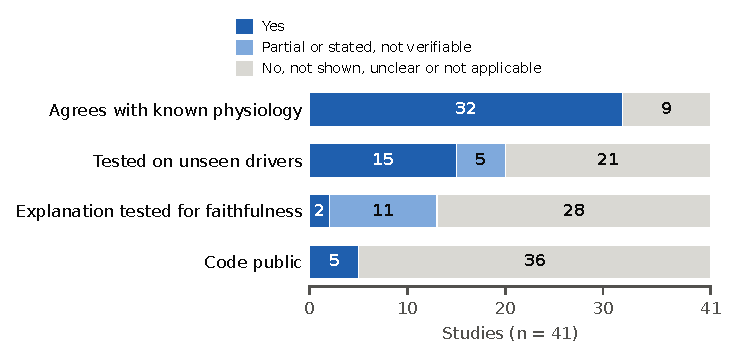
\includegraphics[width=\columnwidth]{fig2_appraisal}
\caption{Appraisal of the 27 detection studies on four checks. Counts describe the examined set, not the whole field; per-study ratings are in Tables~\ref{tab:eeg}--\ref{tab:vision}.}
\label{fig:appraisal}
\end{figure}

\subsection{Accuracy depends on the test scheme}
An explanation of a model that has memorised its test drivers has limited value, so the test scheme bears directly on RQ3. Fig.~\ref{fig:validation} plots reported accuracy by scheme. The median is 97.5\% under random or within-subject splits and 77.1\% on unseen drivers. The tasks and datasets differ, so this comparison is only descriptive, but the same pattern appears within single studies: 96.9\% to 50.8\% for Seo \textit{et al.}~\cite{seo2025driver}, 97.47\% to 85.43\% for Zhou \textit{et al.}~\cite{zhou2026sedriven}, and 97.2\% to 92.4\% for Rafy \textit{et al.} when moving to another dataset \cite{rafy2026domain}. On UTA-RLDD, a subject-independent baseline reached 65.2\% at video level, with human observers at 57.8\% \cite{ghoddoosian2019realistic}; later papers report about 97\% on the same data with image-level splits, although on a simpler two-class task \cite{rafy2026domain}.

The effect is not uniform. In Hasan \textit{et al.}~\cite{hasan2024validation}, leave-one-participant-out reached 80.1\%, close to a single hold-out split (81.3\%) and above their noisy 10-fold results, on a small dataset of 156 observations. Variance also matters: subject-level means can hide failure on individual drivers, such as the 47.3\% worst case behind a 90.7\% mean in Nomura \textit{et al.}~\cite{nomura2025drowsiness}. Several EEG results also report the best epoch selected on test-fold accuracy \cite{cui2022eeg,cui2022compact,cui2021subject,feng2025id3rsnet}, which is mildly optimistic.

\begin{figure}[!t]
\centering
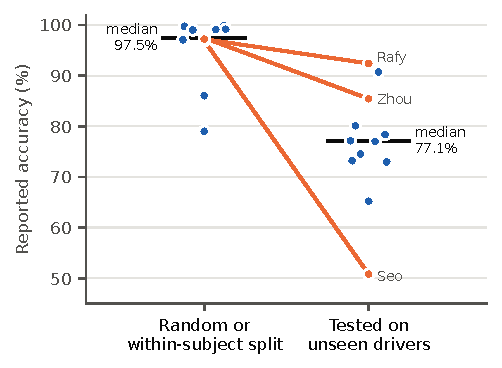
\includegraphics[width=\columnwidth]{fig3_validation}
\caption{Reported accuracy by test scheme, descriptive only because tasks differ. Orange lines join results from one study. Left: \cite{seo2025driver,zhou2026sedriven,gao2025idsrn,alarnaout2025exploiting,mcdonald2014steering,rafy2026domain,florez2023cnn,florez2024realtime,hassan2025realtime,albadawi2023realtime,ersoy2026improving}. Right: \cite{cui2022eeg,cui2022compact,cui2021subject,feng2025id3rsnet,seo2025driver,jiang2026eeg,zhou2026sedriven,hasan2024validation,puspasari2026predicting,rafy2026domain,nomura2025drowsiness,ghoddoosian2019realistic}. Studies with unverifiable splits are omitted.}
\label{fig:validation}
\end{figure}

\subsection{Explanations inherit the label}
Labels limit what any explanation can mean. Four recurring problems appear in the reviewed set.

\textit{Labels derived from model inputs.} AlArnaout \textit{et al.}~\cite{alarnaout2025exploiting} label windows using heart-rate change and level, while mean RR, the inverse of heart rate, is an input. Albadawi \textit{et al.}~\cite{albadawi2023realtime} generate labels from thresholds on the same eye, mouth and head features the classifier receives. High accuracy then partly measures whether the model can recover the rule.

\textit{Eye state as drowsiness.} When the label is open versus closed \cite{florez2023cnn,florez2024realtime,hassan2025realtime,ersoy2026improving}, a heatmap on the eye confirms the definition.

\textit{Time on task as fatigue.} Labels from session order \cite{puspasari2026predicting} or task stage \cite{jiang2026eeg} cannot separate fatigue from anything else that changes over a session.

\textit{Eye signals in the input and the label.} PERCLOS labels combined with EOG input or without eye-artefact removal \cite{zhang2024multimodal,zhou2026sedriven,gao2025idsrn} may let a model detect eye closure directly. Zhou \textit{et al.} raise this risk themselves and test it through frontal-channel removal \cite{zhou2026sedriven}.

By contrast, McDonald \textit{et al.}~\cite{mcdonald2014steering} use video-rated drowsiness with a steering-only model, and Nomura \textit{et al.}~\cite{nomura2025drowsiness} and Ghoddoosian \textit{et al.}~\cite{ghoddoosian2019realistic} use ratings independent of the model's computed features. These give their explanations a firmer footing.

\subsection{Case study: testing one interpretable model and its explanations}
\label{sec:casestudy}
Published accuracy for interpretable EEG models often assumes a protocol that a vehicle cannot follow. Cui \textit{et al.} note that their compact model's batch normalisation uses the whole test subject at once, and that about 6\% of its accuracy depends on this \cite{cui2022compact}. We measured the effect on the multi-channel InterpretableCNN \cite{cui2022eeg}, using our own implementation of its training recipe on the balanced 11-subject subset (2{,}022 samples) under leave-one-subject-out, with five seeds.

Table~\ref{tab:casestudy} shows the results. With statistics from the whole held-out subject, the model reaches 77.93\%, close to the published 78.35\%. Scoring windows one at a time with the same design, as a live system must, gives a constant output (50.00\%, AUC 0.498). Training with running statistics restores a usable streaming model at 73.68\%, which is 4.25 points below the whole-subject figure (better on 9 of 11 subjects for the whole-subject protocol, Wilcoxon $p = 0.042$). On all 27 subjects of the original dataset, using our own conversion of the data, the streaming model reaches 73.59\% balanced accuracy and an AUC of 0.828, so the figure is not specific to the subset.

For comparison, the deep model DeltaGateNet reports 83.21\% on this subset with subject-level five-fold splits \cite{po2026deltagatenet}. Under leave-one-subject-out we obtained 64.74\%, but this is a single seed and a different split, so it is preliminary and is not a direct replication.

\textit{Attribution tests.} We then tested explanations of the two InterpretableCNN variants on every held-out window (five seeds, 11 subjects; all tests across subjects are two-sided Wilcoxon signed-rank tests). Retraining reproduced the accuracies in Table~\ref{tab:casestudy} exactly. We compared saliency, gradient$\times$input, integrated gradients (zero baseline, 50 steps) and CAM with CNN-Fixation tracing, the method published with this model \cite{cui2022eeg}, each explaining the logit margin of the predicted class with normalisation statistics held fixed. The peripheral channel set and the frequency bands were fixed before any results were seen. Code and per-subject results are at \url{https://github.com/sunnyyadav3339/Driver-Drowsiness-Detection-from-EEG}. \todo{True only after research/ is pushed.}

\textit{The decision depends on other windows.} A heatmap explains one window, but under whole-subject normalisation the decision also depends on the driver's other windows. Table~\ref{tab:context} measures this by rescoring the same windows with the same weights and changing only the statistics; labels were used only to build the contexts. Statistics from 30 random windows nearly reproduce the whole-subject result, with 4.80\% of predictions changing. Statistics from alert windows alone change 24.55\% of predictions and raise the predicted-drowsy share from 45.59\% to 68.21\%, and the maps drift far from the baseline (similarity 0.502). A sample-level heatmap shows none of this dependence.

\textit{Faithfulness and sanity can disagree.} Table~\ref{tab:faith} and Fig.~\ref{fig:xaitests} show that every method beat random deletion on at least 10 of 11 subjects ($p \le 0.002$), including the published tracing method, which the EEG comparison of Cui \textit{et al.}~\cite{cui2023towards} did not evaluate. Gradient$\times$input and integrated gradients were strongest under point deletion. This result needs caution: in a nearly piecewise-linear network, removing the points with the largest positive first-order contribution should lower the margin almost by construction, and zeroing takes EEG outside its normal distribution. Channel deletion is more conservative, and there the gap narrows (0.50 against 0.56 for tracing). The same two methods are the weakest on the sanity check: their maps keep a rank correlation of about 0.51 with maps from a randomly initialised network, against 0.13 for saliency and 0.17 for tracing. Multiplying by the input carries amplitude structure into the map whatever the weights are, as Adebayo \textit{et al.} caution \cite{adebayo2018sanity}. Saliency beat random here, unlike in Cui \textit{et al.}~\cite{cui2023towards}, although the procedures differ. No method wins on every test, so reporting one test alone can mislead. Maps were also only moderately stable: channel maps from identical data and different seeds correlated at 0.56 for tracing and 0.72--0.75 for the others.

\textit{What the model uses.} Fig.~\ref{fig:xaitests}(c) and Fig.~\ref{fig:scalp} give the all-window picture for the whole-subject model. Removing theta, alpha or delta lowered P(drowsy) by 0.24, 0.17 and 0.09 on all 11 subjects ($p = 0.001$), and zeroing the 15 central channels lowered it by 0.41. This supports the drowsy reading. Spatially, tracing also agrees with the published alert reading: it placed 64.0\% of alert relevance on the 15 peripheral channels against 45.6\% for drowsy ($p = 0.007$), peaking at F7 for alert and at PZ and CPZ for drowsy. Gradient$\times$input shows a smaller difference (51.9\% against 46.2\%, $p = 0.010$).

On this subset, perturbation does not confirm the alert reading. Zeroing the peripheral channels barely changed P(alert) ($-0.007$, $p = 0.58$), and removing beta had no significant effect ($+0.008$, $p = 0.28$); only gamma removal lowered it, slightly ($-0.036$, $p = 0.001$). Across all windows of this subset, the model behaves like a detector of central low-frequency evidence, with alertness close to the absence of that evidence plus a small high-frequency contribution. Results for the running-statistics variant are similar. These findings qualify the artefact reading but do not refute it. Removing signal also lowers its energy, which may itself favour the alert class. Muscle activity is broadband, so band removal cannot isolate it, and averages can hide windows that behave as the published examples do. The analysis covers one model and 11 subjects, and we did not correct for multiple comparisons, so it should be treated as descriptive evidence.

\textit{The full dataset gives a clearer answer.} We repeated the removal tests with the running-statistics model on all 27 subjects of the original dataset, using our own conversion with natural class balance (five seeds, labelled trials from the 31st of each session). Zeroing the peripheral channels lowered P(alert) by 0.110 ($p < 0.001$), and removing gamma lowered it by 0.074 ($p < 0.001$). The artefact reading therefore has more support on the full dataset than on the 11-subject subset. Here too, removing theta lowered P(drowsy) most among the bands (0.244). The general point stands: a conclusion drawn from inspected samples should be tested across all windows, and here both the test and the choice of data change the conclusion.

\begin{table}[!t]
\centering
\caption{Same Windows and Weights, Different Normalisation Statistics (Whole-Subject Model; Mean over 11 Subjects and 5 Seeds)}
\label{tab:context}
\footnotesize
\begin{tabularx}{\columnwidth}{@{}YL{0.8cm}L{1.15cm}L{1.1cm}L{1.0cm}@{}}
\toprule
\textbf{Statistics from} & \textbf{Acc. (\%)} & \textbf{Changed (\%)} & \textbf{Predicted drowsy (\%)} & \textbf{Map sim.} \\
\midrule
All windows of the subject & 77.93 & 0.00 & 45.59 & 1.000 \\
30 random windows & 77.55 & 4.80 & 45.39 & 0.890 \\
Alert windows only & 68.65 & 24.55 & 68.21 & 0.502 \\
Drowsy windows only & 72.12 & 14.59 & 31.02 & 0.694 \\
\bottomrule
\end{tabularx}
\end{table}

\begin{table}[!t]
\centering
\caption{Attribution Tests on InterpretableCNN. Del.: Area Under the Deletion Curve (Lower Is Better); Sanity: Spearman Correlation with a Randomised Model (Lower Is Better); Stab.: Correlation Across Seeds (Higher Is Better)}
\label{tab:faith}
\footnotesize
\begin{tabularx}{\columnwidth}{@{}YL{0.85cm}L{0.95cm}L{0.8cm}L{0.7cm}@{}}
\toprule
\textbf{Method} & \textbf{Del., points} & \textbf{Del., channels} & \textbf{Sanity} & \textbf{Stab.} \\
\midrule
\multicolumn{5}{@{}l}{\textit{Whole-subject statistics}} \\
CAM + tracing & 0.542 & 0.561 & 0.174 & 0.563 \\
Saliency & 0.580 & 0.641 & 0.128 & 0.754 \\
Gradient$\times$input & 0.185 & 0.501 & 0.513 & 0.719 \\
Integrated gradients & 0.178 & 0.500 & 0.515 & 0.730 \\
Random & 0.667 & 0.707 & -- & -- \\
\midrule
\multicolumn{5}{@{}l}{\textit{Running statistics}} \\
CAM + tracing & 0.563 & 0.584 & 0.167 & 0.603 \\
Saliency & 0.583 & 0.659 & 0.126 & 0.800 \\
Gradient$\times$input & 0.152 & 0.526 & 0.510 & 0.770 \\
Integrated gradients & 0.161 & 0.525 & 0.511 & 0.775 \\
Random & 0.695 & 0.737 & -- & -- \\
\bottomrule
\end{tabularx}
\end{table}

\begin{figure*}[!t]
\centering
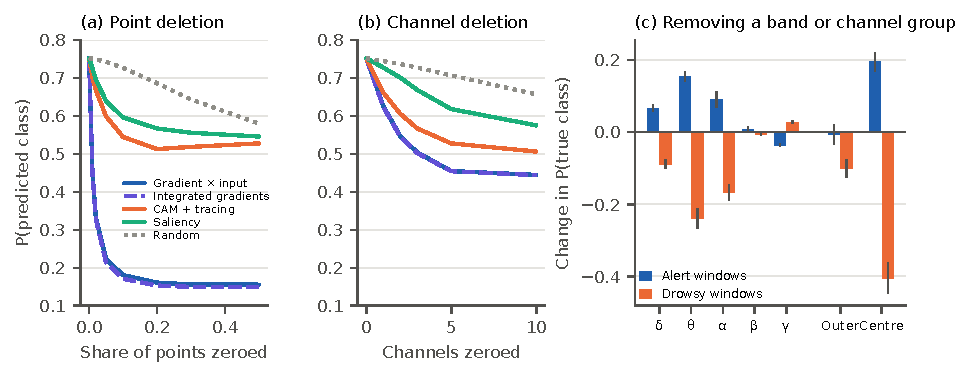
\includegraphics[width=\textwidth]{fig4_xai_tests}
\caption{Tests on the whole-subject model, every held-out window. (a), (b) Probability of the originally predicted class as the top-ranked points or channels are zeroed. (c) Change in the probability of the true class when a frequency band is removed or the 15 outer (peripheral) or 15 central channels are zeroed; bars show the mean over subjects, whiskers the standard error.}
\label{fig:xaitests}
\end{figure*}

\begin{figure}[!t]
\centering
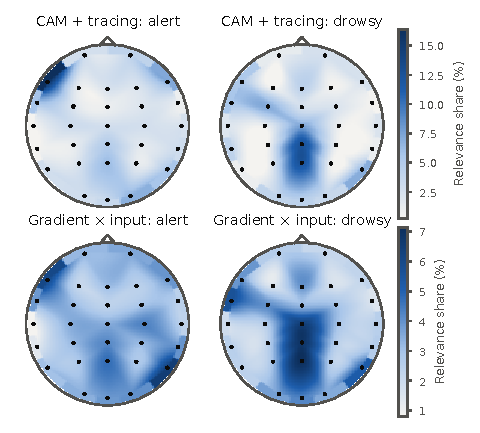
\includegraphics[width=\columnwidth]{fig5_scalp}
\caption{Share of positive relevance per channel for the whole-subject model, averaged over every held-out window per class, then over seeds and subjects. Each method has its own colour scale. Electrode positions are approximate.}
\label{fig:scalp}
\end{figure}

\begin{table}[!t]
\centering
\caption{Case Study on the 11-Subject Subset, Leave-One-Subject-Out}
\label{tab:casestudy}
\footnotesize
\begin{tabularx}{\columnwidth}{@{}YL{1.0cm}L{0.9cm}L{0.8cm}@{}}
\toprule
\textbf{Model and protocol} & \textbf{Acc. (\%)} & \textbf{AUC} & \textbf{Seeds} \\
\midrule
InterpretableCNN, normalised over whole test subject & 77.93 & 0.835 & 5 \\
InterpretableCNN, same, scored one window at a time & 50.00 & 0.498 & 5 \\
InterpretableCNN, running statistics, one window at a time & 73.68 & 0.818 & 5 \\
Band power + logistic regression, one window at a time & 67.14 & 0.743 & 1 \\
DeltaGateNet, one window at a time (preliminary) & 64.74 & 0.766 & 1 \\
EEGNet, one window at a time & 63.85 & 0.752 & 5 \\
\bottomrule
\end{tabularx}
\end{table}

\section{Challenges and Future Directions}
\label{sec:challenges}

\textit{Artefacts and shortcuts.} In the EEG studies we examined, authors repeatedly read alert decisions as muscle, eye and drift signals, and our all-window tests give weak support on the 11-subject subset and clearer support on all 27 subjects (Section~\ref{sec:casestudy}). Occlusion evidence for beta in alert decisions \cite{zhuang2024connectivity} and gamma-led attention at temporal sites \cite{gao2024sftnet} add to the question, since both are hard to separate from muscle activity without further tests. Future work should test whether a model survives artefact removal, a different sensor or a new site, and should state which signals it is meant to use. Comparing explanations with and without artefact removal would be a direct test.

\textit{Testing attention and other built-in explanations.} Attention and learned graphs are now a common interpretability claim in recent EEG work \cite{an2024attention,zhuang2024connectivity,gao2024sftnet,xu2026dynamic}, and the one direct conflict we found \cite{gao2024sftnet} shows why they should not be reported as importance without a test. Occluding the attended bands or channels in the original model would answer this more directly than retraining on single bands.

\textit{Better tests for each modality.} Deletion by zeroing pushes EEG out of its normal distribution, zeroing keypoints creates unrealistic poses \cite{zeynalpour2025multimethod}, and baselines for integrated gradients are a design choice. Vision has a cheap test that none of the reviewed papers ran: mask the eyes and check whether accuracy holds, which would directly test claims of a physiological signal beyond eye closure \cite{nomura2025drowsiness}. Randomisation sanity checks \cite{adebayo2018sanity} are also cheap and were absent from every reviewed study. Our case study and the fidelity comparison of Zeynalpour \textit{et al.}~\cite{zeynalpour2025multimethod} both show that methods rank differently on different tests, so more than one test should be reported.

\textit{Stability across drivers.} A useful explanation should hold on drivers the model has not seen. Most studies explain a few correctly classified samples, or class averages \cite{gao2024sftnet,wu2024driver}. Few report explanation results across all subjects or for errors, and the robustness of explanations under perturbation is untested \cite{vitorino2023adversarial}.

\textit{Attribution for raw cardiac and vehicle signals.} We found no attribution on raw ECG or steering signals in the reviewed set. Redundant HRV features complicate SHAP, so grouping correlated features, or removing them before explanation, should be standard. Vehicle-only explanation is promising but has not yet been shown on unseen drivers \cite{zhu2025madfm}.

\textit{Multimodal attribution.} Fusion models should report how much each modality contributes, in a way that does not simply reward the modality with more features. Attention over modalities is a natural display \cite{theivadas2025dynamic}, but no verifiable study yet tests it, and modality ablation has not been connected to SHAP rankings \cite{guan2025fatigue}.

\textit{Transparent models as a real alternative.} Following Rudin \cite{rudin2019stop}, rule-based and personalised threshold systems deserve serious evaluation. Personalising thresholds improved eye and yawn classification by 1.3--1.5 points in one preprint, narrowing part of the gap to a CNN \cite{ersoy2026improving}. Interpretability constraints on fuzzy sets \cite{yan2026toward} make readability checkable, and could be applied to fuzzy classifiers whose rules are currently unreadable \cite{gao2025comprehensive}. Ontologies add traceable reasoning \cite{georgiadis2026timeaware}. All of these still need valid labels and quantitative tests on real drowsiness, because no reviewed study offers both a readable decision and a verified detection result on unseen drivers.

\textit{Explanations in the control loop.} Once a fatigue estimate sets steering authority \cite{hu2026human,yan2026toward}, an error changes the vehicle's behaviour and not only an alarm. This strengthens the case for readable estimators, but it also raises the bar, because an unvalidated estimate cannot be made safe by being readable. Control studies should validate the estimator separately, on more than a few drivers, and report how the controller behaves when the estimate is wrong.

\textit{Evidence quality and provenance.} Some of the literature cannot be used as evidence at all. We found papers that report no dataset \cite{jha2025realtime}, whose figures disagree with their headline metrics \cite{oise2026enhancing}, whose reported features are not among the described signals \cite{theivadas2025dynamic}, or that report identical results tables under different author lists and no named dataset \cite{sasikala2026robust,nayomi2026vision}. Reviews that only count XAI use would count all of these. Screening for data provenance and duplicated results should precede any count.

\textit{People and deployment.} None of the reviewed studies shows, with data, that explanations improve driver or expert understanding or trust. One paper reports a gain in trust without describing a user study \cite{jha2025realtime}. Counterfactual advice also needs care in this domain, because telling a driver to blink less in order to avoid an alarm could teach them to mask genuine drowsiness. Running an explanation on embedded hardware adds latency \cite{rafy2026domain}, and several authors note that demographic coverage is thin or unreported \cite{rafy2026domain,oise2026enhancing,zhu2025madfm,guan2025fatigue}. Drowsiness data are also sensitive personal and physiological information, as Ali \textit{et al.} discuss \cite{ali2026intelligent}.

\subsection{Reporting checklist}
Table~\ref{tab:checklist} lists what we suggest future studies report. Most items cost little, and several could be added to an existing study in a day.

\begin{table}[!t]
\centering
\caption{Suggested Reporting Checklist for XAI Drowsiness Studies}
\label{tab:checklist}
\footnotesize
\begin{tabularx}{\columnwidth}{@{}L{0.42cm}Y@{}}
\toprule
\textbf{\#} & \textbf{Item} \\
\midrule
1 & Name the dataset, subject count and labelling procedure, and confirm that every reported feature exists in the data. \\
2 & Show actual explanation output, including misclassified samples and worst-performing subjects, and test claims drawn from selected samples across all windows. \\
3 & State the mechanism: intrinsic, post-hoc model-specific or post-hoc model-agnostic, and the exact explainer used. \\
4 & Test faithfulness against a random baseline (for example deletion, ROAR or fidelity) and run a sanity check; report more than one test, since they can disagree. \\
5 & Test attention or learned structure before reporting it as importance. \\
6 & Report results on unseen drivers, with splits grouped by person, and give per-subject results. \\
7 & State whether inference needs other samples from the test subject, such as batch normalisation over a session. \\
8 & Keep feature selection, including selection by SHAP, inside training folds, and fix training length without using test-fold accuracy to choose the epoch. \\
9 & Define the label, and state whether it derives from any input signal, from a recording session or from acted behaviour. \\
10 & Describe artefact handling and test its effect on the explanation. \\
11 & Compare explanations with known physiology, say where they disagree, and keep claims within what the sensor layout can resolve. \\
12 & Report explanation stability across folds and subjects. \\
13 & For multimodal or correlated inputs, report contribution in a way that accounts for feature count and redundancy. \\
14 & For rule systems, map rules to named signals, and validate the output against an independent drowsiness measure. \\
15 & Share code and, where possible, data. \\
\bottomrule
\end{tabularx}
\end{table}

\section{Conclusion}
\label{sec:conclusion}

This review examined interpretable and explainable drowsiness detection across modalities. On RQ1, post-hoc methods dominate: the CAM family in vision and single-channel EEG, and SHAP on hand-crafted features in cardiac and multimodal work. Intrinsic approaches exist but are less common.

On RQ2, explanations often recover known signs of drowsiness, such as theta and alpha activity, eye closure and reduced steering activity. They also point to possible shortcuts: muscle and eye artefacts in EEG, a reading our all-window tests support more clearly on all 27 subjects than on the 11-subject subset, and background regions in vision. In several studies, what the explanation shows follows from how the label was defined.

On RQ3, testing is rare. Of the 27 detection studies we appraised, one tested faithfulness quantitatively, seven applied a partial check and 19 did not evaluate the explanation, while 11 clearly tested on unseen drivers. Our case study adds that a test protocol can decide whether a published interpretable model works at all when scored live, that changing only normalisation statistics can alter a quarter of its decisions, and that deletion and sanity checks can rank the same methods in opposite order.

On RQ4, the main obstacles are untested explanations, labels tied to model inputs, narrow datasets and the absence of user studies. Our checklist targets these directly. The main limit of this review is that it covers a targeted selection of 30 papers, so a larger systematic count is a natural next step. Until explanations are tested as rigorously as accuracy, a heatmap should be treated as a hypothesis about a model, not as evidence that the model can be trusted.


\section*{Acknowledgment}
\todo{Thank the supervisor and TA.}

\bibliographystyle{IEEEtran}
\bibliography{references}

\end{document}
